\documentclass[11pt]{article}
\usepackage{emptypage}
\usepackage{cite}
\usepackage{amsmath,amssymb,amsfonts}
\usepackage{caption}
\usepackage{subcaption}
\usepackage{tabularx}
\usepackage{pifont}
\usepackage{siunitx}
\usepackage[explicit]{titlesec}
\usepackage[bookmarks=true]{hyperref}
\usepackage{bookmark}
\usepackage{svg}
\usepackage{amsmath}
\usepackage{listings}
\usepackage{graphicx}
\usepackage{textcomp}
\usepackage{xcolor}
\usepackage{makecell}
\usepackage{float}
\usepackage{stfloats}
\usepackage{authblk}
\usepackage{acro}%by islam
\usepackage[margin=3cm]{geometry}
\usepackage{algorithm2e}
% Drawing
\usepackage{tikz}
% Tikz Library
\usetikzlibrary{calc, quotes, angles}
% Notation
\usepackage{physics, bm}
\usepackage{pgfplots}
\usetikzlibrary{decorations.markings}
\usetikzlibrary{shapes, arrows}


\usepackage{nomencl}
\usepackage{siunitx}
\usepackage{hyperref}
\makenomenclature
\hypersetup{
    colorlinks=true,
    urlcolor=blue,
}
%% This will add the subgroups
%----------------------------------------------
\usepackage{etoolbox}
\renewcommand\nomgroup[1]{%
  \item[\bfseries
  \ifstrequal{#1}{A}{Physics Constants}{%
  \ifstrequal{#1}{B}{Number Sets}{%
  \ifstrequal{#1}{C}{Other Symbols}{}}}%
]}
%----------------------------------------------

%% This will add the units
%----------------------------------------------
\newcommand{\nomunit}[1]{%
\renewcommand{\nomentryend}{\hspace*{\fill}#1}}
%----------------------------------------------


















\title{Space Systems Engineering Assignment 3}
\author[1]{Mohamed Fawzi}
\author[2]{Islam Zaid}
\affil[1]{Aerospace Department, Khalifa University\\100064444@ku.ac.ae}
\affil[2]{Aerospace Department, Khalifa University\\islam.zaid@ku.ac.ae}
\date{}





% \begin{acronym}[IFR] % Give the longest label here so that the list is nicely aligned
% \acro{IFR}{Inertial Frame of Reference}
% \acro{TLA}{Three Letter Acronym}
% \end{acronym}

\DeclareAcronym{IFR}{
  short=IFR,
  long=Inertial Frame of Reference,
}

\DeclareAcronym{FOV}{
  short=FOV,
  long=Field of View,
}

%%%%%%%%%%%%%%%%%%%%%%%%%%%%%%%%%%%%%%%%%%%%%%%%%%%%%%%%%%%%%%%%%%%%
\begin{document}
\maketitle


\section{Introduction} MSF
\indent

Orbital elements (don't forget material and properties of sat)
Objective
The thermal factors that affect a satellite

\newpage



%%%%%%%%%%%%%%%%%%%%%%%%%%%%%%%%%%%%%%%%%%%%%%%%%%%%%%%%%%%%%%%%%%%%%%%%%%%%%%%%
\section{Methodology} IZ  %%%%%%%%%%%%%%%%%%%%%%%%%%%%%%%%%%%%%%%%%%%%%%%%%%%%%%
%%%%%%%%%%%%%%%%%%%%%%%%%%%%%%%%%%%%%%%%%%%%%%%%%%%%%%%%%%%%%%%%%%%%%%%%%%%%%%%%
\indent
\subsection{Dynamics and Celestial Mechanics}

(see Chapter 3), it provides us with the theoretical framework for celestial
mechanics. The orbits that it forecasts will be relative to an Inertial Frame of Reference
(IFR) that is fixed with respect to the stars; the consequential motion relative to the ground
will also be covered in Chapter 5.

Kepler laws:
These are
1. the orbit of each planet is an ellipse with the Sun occupying one focus;
2. the line joining the Sun to a planet sweeps out equal areas in equal intervals of time;
3. a planet’s orbital period is proportional to the mean distance between the Sun and the
planet, raised to the power 3/2.\\

\paragraph{\ac{IFR}} 
The \ac{IFR} is fixed with respect the sun, where the origin of the axes is the center of the sun. This \ac{IFR} is defined by three unit vectors $\vec{i}, \vec{j}, \vec{k}$ as shown in Figure \ref{fig:ifr}. $\vec{k}$ is normal to the paper and pointing out.

 
\begin{figure}[h]
 
\centering
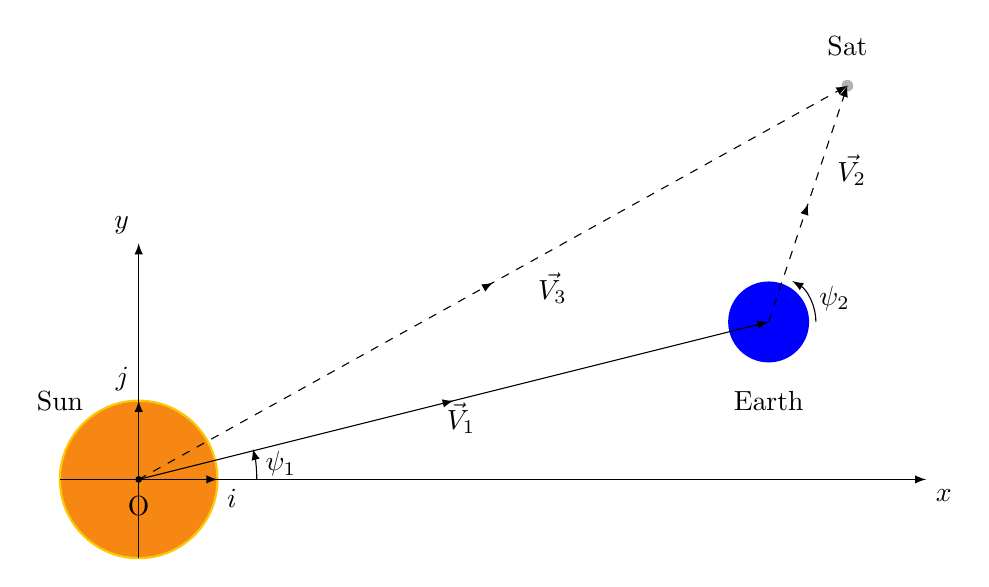
\begin{tikzpicture}[>=latex, decoration={markings, mark=at position 0.5 with {\arrow{>}}}]
    % Coordinates
    \coordinate (sun) at (0,0);
    \coordinate (earth) at (8,2);
    \coordinate (sat) at (9,5);
    \coordinate (A) at (-1,1);
    \coordinate (B) at (8,1);
    \coordinate (C) at (9,5.5);
    
    % Earth
    \draw[thick, fill=yellow!50!red, draw=yellow!80!red] (sun) circle (1);
    % Text
    \node (a) at (A) {Sun};

    % Earth
    \draw[thick, fill=blue, draw=blue] (earth) circle (0.5);
    % Text
    \node (b) at (B) {Earth};
    
    % Moon
    \node[circle, inner sep=1.5pt, outer sep=2pt, fill=black!30] (MOON) at (sat) {};
    % Text 
    \node (c) at (C) {Sat};
    
    % Lines
    \draw[-latex, postaction={decorate}] (sun) -- (earth) node[pos=.55, below left] {$\vec{V}_{1}$};
    \draw[dashed, -latex, postaction={decorate}] (earth) -- (sat) node[pos=.75, below right] {$\vec{V_2}$};
    \draw[dashed, -latex, postaction={decorate}] (sun) -- (sat) node[pos=.55, below right] {$\vec{V_3}$}; 
    
    % Angles
    \draw[->] (sun) ++(0:1.5) arc (0:15:1.5) node[midway, right] {$\psi_1$};
    \draw[->] (earth) ++(0:0.6) arc (0:60:0.6) node[midway, right] {$\psi_2$};
    
    % Point
    \draw[fill=black] (sun) circle (1pt) node[below, shift={(0,-0.1)}] {$\mathrm{O}$};

    % X and Y axes
    \draw[-latex] (-1,0) -- (10,0) node[below right] {$x$};
    \draw[-latex] (0,-1) -- (0,3) node[above left] {$y$};
    % i and j axes
    \draw[-latex] (0,0) -- (1,0) node[below right] {$i$};
    \draw[-latex] (0,0) -- (0,1) node[above left] {$j$};
\end{tikzpicture}
\caption{\ac{IFR} and vector position of the Earth, and satellite}
\label{fig:ifr}
\end{figure}


 
 
\paragraph{Position vector of the earth wrt the sun ($\vec{V_1(\psi_1)}$),}

the vector from the sun to the earth is $\vec{V}_{1}$, which consists of three components in $X, Y, \text{and } Z$ directions. %the initial position of the satellite at $t_0 = 0$ is represented by 
\begin{equation}\label{eq:01}
    \vec{V}_{1}(\psi_{1}) = (r_{1}(\psi_1)) \vec{i} + (0) \vec{j} + (0) \vec{k}\end{equation}
$r_{1}(\psi)$ is the distance between the sun and earth at an angle ($\psi$).

Rotation matrix [$R$] is used to rotate $\vec{V}_{1}$ around the origin of the axes. it results from the multiplication of three rotation matrices ($[R_x], [R_y], \text{ and } [R_z]$) These matrices are 
\begin{equation}
[R_x(\phi)] = \begin{bmatrix}
            1 &0 & 0 \\
            0 & \cos{\phi}& -\sin{\phi} \\
            0 & \sin{\phi}&\cos{\phi}
            \end{bmatrix}
[R_y(\theta)] = \begin{bmatrix}
            cos{\theta} &0 & \sin{\theta} \\
            0 & 1& 0 \\
            -\sin{\theta}&0 & \cos{\theta}
            \end{bmatrix}
[R_z(\psi)] = \begin{bmatrix}
            cos{\psi}  &  -\sin{\psi}  &  0    \\
            \sin{\psi}&   \cos{\psi}    & 0\\
            0          &    0   & 1          
            \end{bmatrix}        
\end{equation}

\begin{equation}\label{eq:11}
[R(\phi, \theta, \psi)]= [R_z(\psi)][R_y(\theta)][R_x(\phi)]
\end{equation}


Since this study targets a simplified model, where the satellite is limited to rotating in the equatorial plane only. Then, no rotation about X, and Y directions. 
Consequently,
\begin{equation}\label{fig:6}
    \phi(t) = \theta(t) = 0 
    \end{equation}
\begin{equation}\label{eq:7}
    [R_x(\phi(t))]=[R_y(\theta(t))]=[eye] .
\end{equation}
By substitution from Eq \ref{eq:11} into Eq \ref{eq:7},
\begin{equation}\label{eq:04}
    [R(\phi, \theta, \psi)] = [eye] [ eye] [R_z(\psi_1(t))]
\end{equation}
\begin{equation}\label{eq:04}
    [R(\psi)] = [R_z(\psi_1(t))]
\end{equation}

\begin{equation}\label{eq:05}
    \vec{V}_1(\psi_1) = [R(\psi_1)] \vec{V}_1(\psi_1)  
\end{equation}

By substitution from Eq \ref{eq:01}, and Eq \ref{eq:04} into Eq \ref{eq:05}

\begin{gather}\label{eq:06}
\vec{V}_1(t) = \begin{bmatrix}
            cos{\psi_1(t)}  &  -\sin{\psi_1(t)}  &  0    \\
            \sin{\psi_1(t)}&   \cos{\psi_1(t)}    & 0\\
            0          &    0   & 1          
            \end{bmatrix}  \begin{bmatrix}
            r_1(t)   \\
            0 \\
             0             
            \end{bmatrix}  
            = \begin{bmatrix}
            r_1(t) . cos{\psi_1(t)}  \\
            r_1(t) . sin{\psi_1(t)} \\
             0             
            \end{bmatrix}
\end{gather}

\paragraph{Position vector of the satellite wrt the earth ($\vec{V_2(t)}$),}


Similarly, the satellite is rotating around the earth according to the same governing equations. Considering that the satellite is rotating in a circular path. Then, $r_2(t) = r_2$. Thus,
\begin{equation}
    \vec{V}_2(t) = \begin{bmatrix}
            cos{\psi_2(t)}  &  -\sin{\psi_2(t)}  &  0    \\
            \sin{\psi_2(t)}&   \cos{\psi_2(t)}    & 0\\
            0          &    0   & 1          
            \end{bmatrix}  \begin{bmatrix}
            r_2   \\
            0 \\
             0             
            \end{bmatrix}  
            = \begin{bmatrix}
            r_2 . cos{\psi_2(t)}  \\
            r_2 . sin{\psi_2(t)} \\
             0             
            \end{bmatrix}
\end{equation}
\paragraph{Position vector of the satellite wrt the sun ($\vec{V_3(t)}$),}

It is evident from geometry of Figure \ref{fig:ifr} that,
\begin{equation}
    \vec{V_3}(t) = \vec{V_1}(t) + \vec{V_2}(t)
\end{equation}
\begin{equation}
    \vec{V}_3(t)  = 
            \begin{bmatrix}
            r_1(t) . cos{\psi_1(t)}  \\
            r_1(t) . sin{\psi_1(t)} \\
             0             
            \end{bmatrix} 
            +
            \begin{bmatrix}
            r_2 . cos{\psi_2(t)}  \\
            r_2 . sin{\psi_2(t)} \\
             0             
            \end{bmatrix}  
\end{equation}
\begin{equation}
    \vec{V}_3(t)  =  
            \begin{bmatrix}
            r_1(t) . cos{\psi_1(t)} +r_2 . cos{\psi_2(t)}  \\
            r_1(t) . sin{\psi_1(t)} +r_2 . sin{\psi_2(t)} \\
             0                                
            \end{bmatrix} 
\end{equation}


\paragraph{Orbital Elements}


Two-body problem solution of earth-sun system\cite{fortescue2011spacecraft}.  
 

In this project, the time will be considered as the dependent variable. Thus, the independent variable should be calculated as follows;

\begin{figure}[h]
\centering
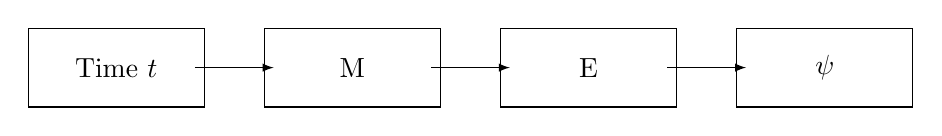
\begin{tikzpicture}
% draw rectangle node
	\node[draw,
		minimum width=2cm,
		minimum height=1cm,
		align=center,
		text width=2cm] at (0,0) {Time $t$};
	\node[draw,
		minimum width=2cm,
		minimum height=1cm,
		align=center,
		text width=2cm] at (3,0) {M};
	\node[draw,
		minimum width=2cm,
		minimum height=1cm,
		align=center,
		text width=2cm] at (6,0) {E};
	\node[draw,
		minimum width=2cm,
		minimum height=1cm,
		align=center,
		text width=2cm] at (9,0) {$\psi$};

    \draw[-latex] (1,0) -- (2,0);
    \draw[-latex] (4,0) -- (5,0);
    \draw[-latex] (7,0) -- (8,0);
\end{tikzpicture}
\caption{Your caption here}
\label{fig:2}
\end{figure}

According to the sequence in Figure \ref{fig:2}, the angular position ($\psi$) of the orbital objects could be calculated as a function of a given time (t).

\begin{gather}\label{eq:12}
    M = n t \\
    E-e\sin{E} = M \\
    \tan{\psi/2} = \tan{E/2}\sqrt{\frac{1+e}{1-e}} \\
\end{gather}

Also, the position on the ellipse (r) may be written in terms of ($\psi$) as
\begin{gather}\label{eq:14}
    r = \frac{h^2/\mu}{1+e\cos{\psi_1}}\\
    h^2/\mu = a(1-e^2)
\end{gather}

The periodic time ($\tau$),
 
\begin{equation}
    \tau = 2\pi\sqrt{a^3/\mu}
\end{equation}



\subsection{Thermal Models}

\paragraph{Solar radiation,} The solar is emitting a constant amount of traditional power ($P$) equals \SI{3.856e26}{\watt}. The Solar radiation flux of a point at a distance ($d$) from the center of the earth could be calculated according to Eq \ref{eq:solarflux}.

\begin{equation} \label{eq:solarflux}
    J_s = \frac{P}{4\pi d^2}
\end{equation}



\begin{figure}[h]
 
\centering
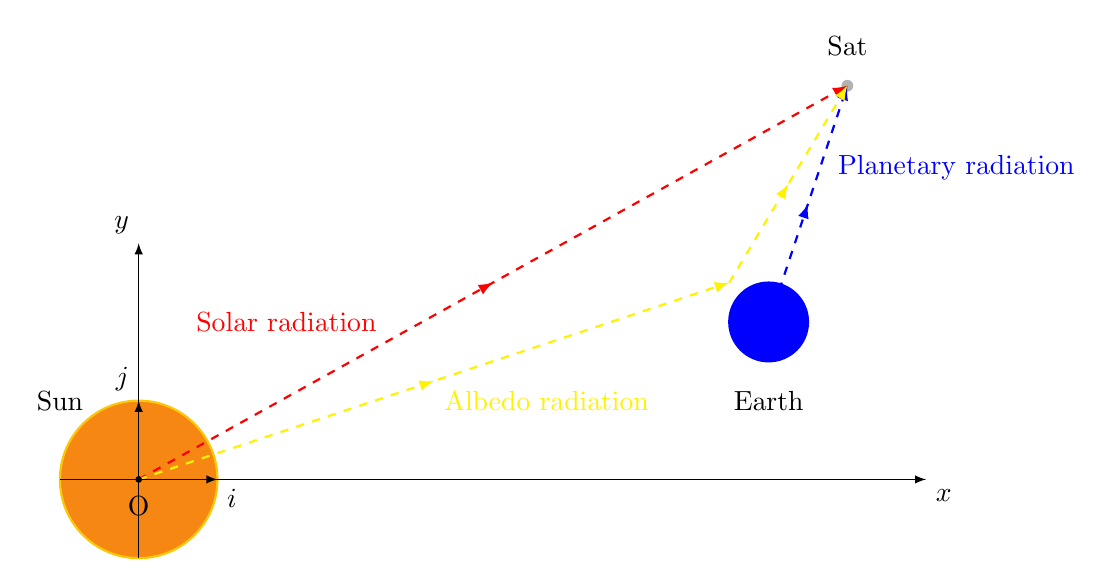
\begin{tikzpicture}[>=latex, decoration={markings, mark=at position 0.5 with {\arrow{>}}}]
    % Coordinates
    \coordinate (sun) at (0,0);
    \coordinate (earth) at (8,2);
    \coordinate (sat) at (9,5);
    \coordinate (A) at (-1,1);
    \coordinate (B) at (8,1);
    \coordinate (C) at (9,5.5);
    
    % Earth
    \draw[thick, fill=yellow!50!red, draw=yellow!80!red] (sun) circle (1);
    % Text
    \node (a) at (A) {Sun};

    % Earth
    \draw[thick, fill=blue, draw=blue] (earth) circle (0.5);
    % Text
    \node (b) at (B) {Earth};
    
    % Moon
    \node[circle, inner sep=1.5pt, outer sep=2pt, fill=black!30] (MOON) at (sat) {};
    % Text 
    \node (c) at (C) {Sat};
    
    % Lines
    % \draw[-latex, postaction={decorate}] (sun) -- (earth) node[pos=.55, below left] {$\vec{V}_{1}$};
    \draw[dashed, -latex, postaction={decorate},blue,thick] (earth) -- (sat) node[pos=.75, below right] {\textcolor{blue}{Planetary radiation}};
    \draw[dashed, -latex, postaction={decorate},red,thick] (sun) -- (sat) node[pos=.35, above left] {\textcolor{red}{Solar radiation}}; 
    \draw[dashed, -latex, postaction={decorate},yellow,thick] (sun) -- (7.5,2.5) node[pos=.5, below right] {\textcolor{yellow}{Albedo radiation}}; 
    \draw[dashed, -latex, postaction={decorate},yellow,thick] (7.5,2.5) -- (sat) node[pos=.5, below right] {}; 
    
    % Angles
    % \draw[->] (sun) ++(0:1.5) arc (0:15:1.5) node[midway, right] {$\psi_1$};
    % \draw[->] (earth) ++(0:0.6) arc (0:60:0.6) node[midway, right] {$\psi_2$};
    
    % Point
    \draw[fill=black] (sun) circle (1pt) node[below, shift={(0,-0.1)}] {$\mathrm{O}$};

    % X and Y axes
    \draw[-latex] (-1,0) -- (10,0) node[below right] {$x$};
    \draw[-latex] (0,-1) -- (0,3) node[above left] {$y$};
    % i and j axes
    \draw[-latex] (0,0) -- (1,0) node[below right] {$i$};
    \draw[-latex] (0,0) -- (0,1) node[above left] {$j$};
\end{tikzpicture}
\caption{Radiation modes}
\label{fig:ifr}
\end{figure}

\paragraph{Albedo radiation} 
The portion of solar radiation that bounces off a planet's surface and/or atmosphere. this fraction (a) is in range (0.31 - 0.39). 
\begin{equation}
    \delta Q_{r_{ij}} = I_{i0} dA_i\cos{\phi_i}\times\frac{dA_j \cos{\phi_j}}{d^2}
\end{equation}

\paragraph{Planetary radiation} 



































Albedo
Solar Radiation
Planetary
Emission (we need to further look into it)

\subsection{Positioning} %%%%%%Needs to change%%%%%%%
Mathematical approach
explanation of each vector
implementation of vectors with time
discretization 
Earth model, and coordinates

\RestyleAlgo{ruled}

%% This is needed if you want to add comments in
%% your algorithm with \Comment
\SetKwComment{Comment}{/* }{ */}

\begin{algorithm}[hbt!]
\caption{An algorithm with caption}\label{alg:two}
\KwData{$n \geq 0$}
\KwResult{$y = x^n$}
$y \gets 1$\;
$X \gets x$\;
$N \gets n$\;
\While{$N \neq 0$}{
  \eIf{$N$ is even}{
    $X \gets X \times X$\;
    $N \gets \frac{N}{2} $ \Comment*[r]{This is a comment}
  }{\If{$N$ is odd}{
      $y \gets y \times X$\;
      $N \gets N - 1$\;
    }
  }
}
\end{algorithm}



\newpage
\section{Results} %MSF&IZ
\indent
FOR EACH MATERIAL (EXCEPT ANIMATIONS)
\begin{enumerate}
    \item Temp variance w.r.t earth-sun period
    \item $Q_{s}$,$Q_{a}$ and $Q_{p}$ variance w.r.t earth-sun period
    \item Temp variance w.r.t Sat-earth period
    \item $Q_{s}$,$Q_{a}$ and $Q_{p}$ variance w.r.t sat-earth period
    \item animation of sat-earth
    \item animation of earth-sun 


\end{enumerate}


\newpage
\section{Discussion} %MSF&IZ
\indent

\newpage
\section{Conclusion} MSF
\indent






%%%%%%%%%%
%%%%%%%%%%%
%%%%%%%%%%%%
\nomenclature[A, 01]{$\mu$}{\href{https://en.wikipedia.org/wiki/Standard_gravitational_parameter}{Gravitational Parameter} \nomunit{\SI{3.986e14}{\meter\cubed\per\second\squared}}}
\nomenclature[A, 02]{\(h\)}{\href{https://physics.nist.gov/cgi-bin/cuu/Value?h}
{Planck constant}
\nomunit{\SI[group-digits=false]{6.62607015e-34}{\joule\per\hertz}}}
\nomenclature[A, 03]{\(G\)}{\href{https://physics.nist.gov/cgi-bin/cuu/Value?bg}
{Gravitational constant} 
\nomunit{\SI[group-digits=false]{6.67430e-11}{\meter\cubed\per\kilogram\per\second\squared}}}
\nomenclature[B, 03]{\(\mathbb{R}\)}{Real numbers}
\nomenclature[B, 02]{\(\mathbb{C}\)}{Complex numbers}
\nomenclature[B, 01]{\(\mathbb{H}\)}{Quaternions}
\nomenclature[C]{\(V\)}{Constant volume}
\nomenclature[C]{\(\rho\)}{Friction index}









\printnomenclature
\printacronyms
\bibliography{References}

\end{document}

